% Slides for 2025-08-19
% To create a slide, use the following:
% \begin{frame}{TITLE}
%     BODY
% \end{frame}

% To create a slide with a bullet list, use the following:
% \begin{frame}{TITLE}
%     \begin{itemize}
%         \item ITEM 1
%         \item ITEM 2
%     \end{itemize}    
% \end{frame}

% To create a slide with numbered list, use the following:
% \begin{frame}{TITLE}
%     \begin{enumerate}
%         \item ITEM 1
%         \item ITEM 2
%     \end{enumerate}
% \end{frame}

% To create a slide with a graphic:
% 1. Add the graphic to this folder (named picture.png)
% 2. Use the following:
% \begin{frame}{TITLE}
%     \centering
%     \includegraphics[height=0.7\textheight,width=0.7\textwidth,keepaspectratio]{picture.png}
% \end{frame}

% To create a slide with two columns, use the following:
% \begin{frame}{TITLE}
%     \begin{columns}
%         \begin{column}{0.5\textwidth}
%             COLUMN 1 BODY
%         \end{column}
%         \begin{column}{0.5\textwidth}
%             COLUMN 2 BODY
%         \end{column}
%     \end{columns}
% \end{frame}

\begin{frame}{ML Team Agenda}
    \begin{itemize}
        \item 
    \end{itemize}
\end{frame}

\begin{frame}{Collar Team Agenda}
    \begin{itemize}
        \item Integration
        \item Inference Testing
        \item Power Studies
        \item Auto Encoders       
    \end{itemize}
\end{frame}

\begin{frame}{Integration}
    \begin{itemize}
        \item Real-Time Clock (RTC) configured
        \item Configuring CM4 core to test power as wake-up system
        \item Noise affecting model inferences → new mic/pipeline bypass
    \end{itemize}
\end{frame}

\begin{frame}{Inference Testing}
    \begin{itemize}
        \item Domain shift from microphone 
        \item Heavy noise in mel bands 20-30, 60, even after filtering
    \end{itemize}
    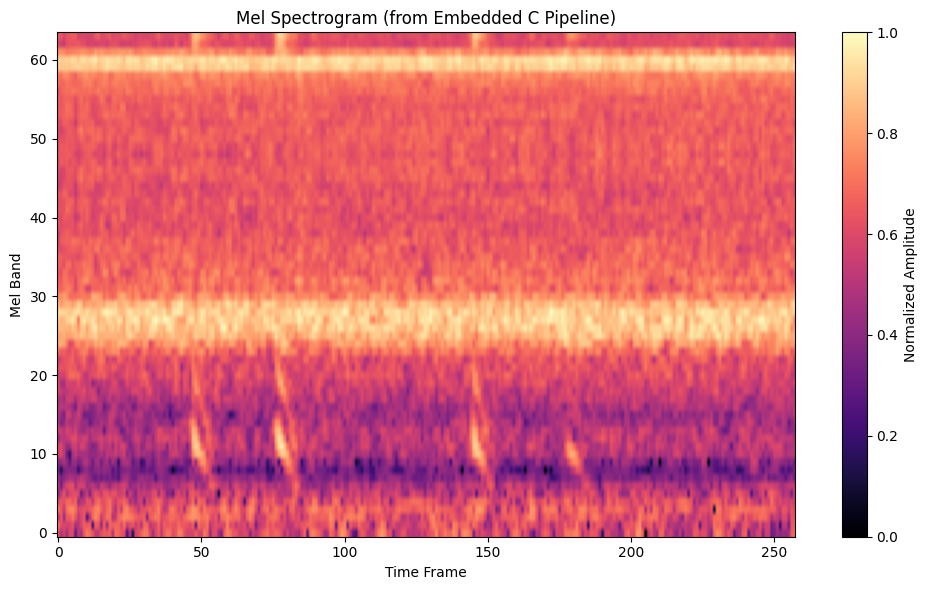
\includegraphics[height=0.7\textheight,width=0.5\textwidth,keepaspectratio]{images/melSpec.png}
    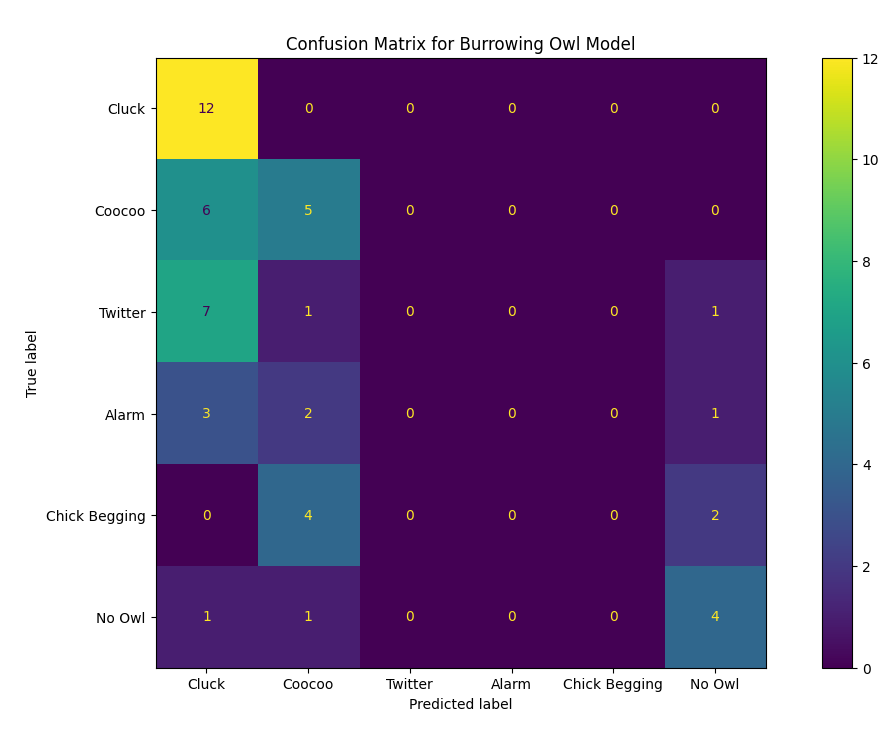
\includegraphics[height=0.7\textheight,width=0.39\textwidth,keepaspectratio]{images/confusionMatrix.png}
\end{frame}

\begin{frame}{Power Studies}
    \begin{itemize}
        \item Testing CM4 core wake-up
        \item Integrated system re-test
        \item Future plans to measure LoRa
    \end{itemize}
    \begin{table}[]
    \begin{tabular}{lll}
    \hline
                & Independent (mA) & Integrated System (mA) \\ \hline
    Baseline       & 13.43            & 6.99                  \\
    Mic            & 23.6             & 10.37                 \\
    Inf + Mel Spec & 16.0             & 12.46                 \\
    MicroSD        & 14.1             & 7.74                  \\
    LoRa          & TBD              & TBD                     \\ \hline
    \end{tabular}
    \end{table}
\end{frame}

\begin{frame}{Auto Encoders}
    \begin{itemize}
        \item 
    \end{itemize}
\end{frame}




